\documentclass[twocolumn]{amsart}
\usepackage[top=0.5in, left=0.45in, right=0.45in, bottom=0.5in]{geometry}

\usepackage{url}
% \usepackage{code}
% \usepackage{cite}
\usepackage{amsmath}
\usepackage{amssymb}
\usepackage{graphicx}
\usepackage{chessboard}

% \usepackage{chessfs}
\usepackage{adjustbox}

% Define black versions of pieces for inline use. Gross, but it works.
\newcommand{\Pawn}[1][1.3ex]{%
\adjustbox{Trim=4.3pt 2.6pt 4.3pt 0pt,width=#1,margin=0.2ex 0ex 0.2ex 0ex}{\BlackPawnOnWhite}%
}%
\newcommand{\Rook}[1][1.58ex]{%
\adjustbox{Trim=3.2pt 2.2pt 3.2pt 0pt,width=#1,raise=0ex,margin=0.1ex 0ex 0.1ex 0ex}{\BlackRookOnWhite}%
}%
\newcommand{\Knight}[1][1.85ex]{%
\adjustbox{Trim=2.3pt 2.35pt 2.5pt 0pt,width=#1,raise=-0.03ex,margin=0.14ex 0ex 0.14ex 0ex}{\BlackKnightOnWhite}%
}%
\newcommand{\Bishop}[1][1.79ex]{%
\adjustbox{Trim=2.3pt 2pt 2.3pt 0pt,width=#1,raise=-0.12ex,margin=0.1ex 0ex 0.1ex 0ex}{\BlackBishopOnWhite}%
}%
\newcommand{\Queen}[1][2.05ex]{%
\adjustbox{Trim=1.2pt 2.2pt 1.2pt 0pt,width=#1,raise=-0.08ex,margin=0.1ex 0ex 0.1ex 0ex}{\BlackQueenOnWhite}%
}%
\newcommand{\King}[1][1.95ex]{%
\adjustbox{Trim=2pt 2pt 2pt 0pt,width=#1,raise=-0.06ex,margin=0.13ex 0ex 0.13ex 0ex}{\BlackKingOnWhite}%
}%

\interfootnotelinepenalty=0

% lets me explicitly set a. or 1. etc. as enum label
\usepackage{enumitem}

\pagestyle{empty}

\usepackage{ulem}
% go back to italics for emphasis, though
\normalem

\usepackage{natbib}

\setlength{\footnotesep}{2em}

% \newcommand\comment[1]{}
\newcommand\sfrac[2]{\!{}\,^{#1}\!/{}\!_{#2}}

\begin{document} 

\title{Color- and piece-blind chess}
\author{Dr.~Tom~Murphy~VII~Ph.D.}\thanks{
Copyright \copyright\ 2019 the Regents of the Wikiplia Foundation.
Appears in The Journal Of LaTeX Class Files with the insufficient
material of the Association for Computational Heresy; {\em IEEEEEE!}
press, Verlag-Verlag volume no.~0x40-2A. 1 tempo}

\setchessboard{showmover=false}

\newcommand\checkmate{\hspace{-.05em}\raisebox{.4ex}{\tiny\bf ++}}

\renewcommand\th{\ensuremath{{}^{\textrm{th}}}}
\newcommand\st{\ensuremath{{}^{\textrm{st}}}}
\newcommand\rd{\ensuremath{{}^{\textrm{rd}}}}
\newcommand\nd{\ensuremath{{}^{\textrm{nd}}}}
\newcommand\at{\ensuremath{\scriptstyle @}}

\date{1 April 2019}

\maketitle \thispagestyle{empty}

% \begin{abstract}
% CHESSMATE.
% \end{abstract}

\section{Impressing humans}

What better way for humans to impress each other with their brains,
especially in movies, than to play chess---and to shout dramatically
CHECKMATE! upon surprise-checkmating their opponent? Well, one way is
to play chess while disadvantaged somehow, for example, by punching
each other in the face repeatedly during the game to impair brain
function (see Chess Boxing~\cite{wikipediachessboxing}). Another
common distraction is to play a multitude of games against many
opponents at the same time, in a so-called ``simultaneous
exhibition.'' The idea is that this is more challenging because of the
need to maintain mental state for so many games at once, whereas your
opponents only need to maintain state for one game. In truth,
simultaneous exhibitions easily fall to a ``man-in-the-middle
attack.'' If the purported genius simply creates a perfect bipartite
matching of the games played with the white pieces and the games
played with black, he can mechanically forward moves between these
pairs of boards. This requires only constant state (see next section)
per pair of games, and guarantees an even score for the exhibition. So
that's not very impressive.

Another disadvantage that humans sometimes use to impress each other
is a blindfold (worn over the eyes). In this predicament they only
hear the opponent announce moves and must imagine the position on the
board in their mind's eye, both for the sake of remembering it and
while exploring potential moves.
% This is effective, since although the .
Disadvantages can be combined, such as in the final scene of the 1988
documentary {\it Bloodsport} where Jean Claude van Damme is blinded by
an illicit foreign substance during the final martial art
battle.\footnote{JCVD does not play chess on camera, but it is implied
  that he is also holding a simultaneous exhibition between rounds in
  a different room of the underground Hong Kong illegal karate
  complex.}
% Note: blindfold simuls are banned in russia as a health hazard!?

\section{Impressing computers}

In contrast, it is much more difficult to impress computers or impress
people with computers. When it comes to computers playing chess,
largely, the jig is up; it is now easy for chess programs, running on
consumer hardware, to defeat the strongest human players. It is well
known that striking a computer actually {\em fixes} it, so Chess
Boxing becomes trivial. Blindfold chess is the natural interface for a
chess computer; it is actually {\em much more difficult} to have the
computer interpret the opponent's move by visually studying a physical
board!

% Computers can still impress us and each other with computational chess
% feats other than playing. For example, computers are largely concerned
% with filling up their memories with efficiently encoded data.

Playing multiple games simutaneously is an easy extension of playing a
single game, although in principle the scale of such a thing could
still be impressive. This is also impressive to other computers, who
are largely concerned with filling up their memories with efficiently
coded data. With a modern chess engine, it is easy to scale
to an arbitrary number of games, since the exhibitor can make progress
by observing one of the boards, computing a strong move, and playing
it; this requires $O(1)$ space because all of the state is stored
externally in the exhibition itself. 
% If playing blindfold, then the
% main cost is storing the state of each game. 
However, we run the risk of losing the tournament (other players may
be yet stronger computers). The man-in-the-middle attack remains an
efficient way to minimize loss (ensuring an exactly even score).
The simplest way to do this is to explicily generate a perfect
bipartite matching over the $n$ games $G$ being played. This consists
of $n/2$ pairs $\langle G_w, G_b \rangle$ (where we play as white
against Bob and black against Walice, respectively). Since each game
starts in the starting position, this is very easy; we can just assign
the matches consecutively. Along with each pair we also record which
of the following states we are in:
\begin{enumerate}
\item We are waiting for a move from Walice (our white opponent) \label{state:mim1}
\item We have seen a move from Walice, which is \underline{\hspace{3em}}. \label{state:mim2}
\item We are waiting for a move from Bob (our black opponent) \label{state:mim3}
\item We have seen a move from Bob, which is \underline{\hspace{6em}}. \label{state:mim4}
\end{enumerate}
If in State~\ref{state:mim1}, we just watch $G_b$ until Walice makes a
move, then record it and proceed to State~\ref{state:mim2}. We consume
the move and move to State~\ref{state:mim3} by playing that move in
$G_w$ against Bob (where it must be our turn). We can immediately seek
out that game or wait until we naturally come upon it. However, we
should only approach $G_w$ when the pair of games is in
State~\ref{state:mim3}, etc., otherwise we will not have a move to play.

There are $n/2$ pairs, with two bits for the state, no more\footnote{
  There are only 1792 pairs of squares between which pieces can ever
  move (Section~\ref{sec:legalmove}), so $11+2$ bits suffices, with
  some added complexity.} than $\log_2(64 \times 64 \times 4) = 14$ bits for
each move (source square, destination square, and 2 bits to
distinguish promotion to queen, rook, bishop, or knight). However, we
also need to store the matching of $G_w$ to $G_b$; this can be done
with a pair of indices (or e.g. memory addresses) but unfortunately,
this requires $\log_2(n)$ bits to represent. So overall this approach
requires $O(n \log(n))$ space to play a simultaneous exhibition of $n$
games.

It appears to be possible to reduce the space usage per game to a
constant. In order to perform a man-in-the-middle attack, we need
a perfect matching between the white games and black games. It is
not essential that the matching be stable over time; for example
if we are forwarding moves between Walice and Bob, and between
Waluigi and Bario, and these games happen to transpose to the same
position, then it works just fine to switch to forwarding between
Walice and Bario; Waluigi and Bob. So, rather than store the
matching explicitly, we can reconstruct it from the stored state
at each step.

Let's think about the process of forwarding the moves from our white
opponents to our black opponents; the reverse is of course symmetric.
The first step will be to wait for the white opponents to make their
moves, and then copy these $n/2$ positions (not moves) into a vector
in memory.

\newcommand\stepsto[1]{\stackrel{#1}{\rightarrow}}
The black opponents are waiting for a move from us. Next, we'll copy
their $n/2$ positions into memory, aligned with the $n/2$ positions
already present. Let's say that the relation that defines a legal
move in chess is
%
$$
B \stepsto{m} B'
$$ 
%
where $B$ is the position before the move $m$, and $B'$ is the
resulting position. Our goal is to align the games such that $B'$ (a
position copied from our white opponent) is aligned with $B$ (a
position pending a move for our black opponent) in memory; this will
represent the perfect matching. Computing $m$ from $B$ and $B'$ when
$B \stepsto{m} B'$ is easy (and unique), so this allows us to read off
and play the move for each row.

By invariant, it will be possible to produce such an alignment. For
example, the first time we do this, each $B$ will be the starting
position, and $B'$ will be a legal move made by white from the
starting position. Any alignment will work. Let's say that just one of
the white opponents played 1. d4, resulting in $B_0$; then one black
opponent will make a legal response to this (say 1. \ldots Nf6, giving
$B_1$). Then $B_1$ can be $B'$ for the next round, which we can align
with $B=B_0$, and so on.

The only tricky thing is figuring out which boards go with which.
Although if $B \stepsto{m} B'$ it is easy to deduce $m$, it is not
possible to compute $B$ from $B'$, or even from $B'$ and $m$. This is
because we may have both $B_a \stepsto{m_a} B'$ and $B_b \stepsto{m_b}
B'$ with $B_a \neq B_b$. For example with $B'$

\chessboard[tinyboard, setfen=k7/8/8/8/8/8/8/K7 w - -, showmover]

\noindent \ldots we could have $B_a$ and $B_b$ be

\chessboard[tinyboard, setfen=Nk6/8/8/8/8/8/8/K7 b - -, showmover]
\chessboard[tinyboard, setfen=Rk6/8/8/8/8/8/8/K7 b - -, showmover]

Both of which can precede $B'$ (the move is even the same: Kxa1).
So it is not enough to greedily assign edges in our perfect match;
if we choose the edge $B_b$ to go with $B'$, we might later find
$B'_2$:

\chessboard[tinyboard, setfen=R7/1k6/8/8/8/8/8/K7 w - -, showmover]

\noindent \ldots and have no possible matching board, since it cannot
legally follow $B_a$.

Fortunately, we know that there exists a perfect matching (assuming
all players are playing legal moves) and we can tell if we found
one (i.e., we didn't get stuck). So, one strategy that works is
to choose randomly when there is some ambiguity, and start over
from the beginning if we ever get stuck. In practice this will
be pretty efficient, since convergent board states are unusual.
We only need a single pseudorandom pool for the entire process,
so it can be $O(n)$ bits; this seems easily enough to generate all
possible permutations of $n/2$ items. Even $2^{2n}$ grows much
faster than $n!$. If we don't like the random approach, I believe
it is also possible to compute \verb+next_permutation+ in
constant space; so we can just explicitly try all orderings for $B'$
(this takes exponential time).

Once we have paired up each $B$ and $B'$, we simply compute the
move (which we now know exists) and play it in that game. We
then wait for the black opponents to play their moves, copy the
resulting board states into our vector and repeat the above
process (but flipping ``black'' and ``white'').

Although this is more involved than the previous approach, and may
take exponential time, it allows us to play against $n$ simultaneous
opponents using $O(n)$ space!
% If the games in the exhibition were presented to us in some way that
% allowed us to visit them in the same order multiple times, we could
% perhaps get away with {\em only} the random pool? XXX

\subsection{Board representations} \label{sec:representation}

The actual space used per game is primarily the representation of
a chess position, plus a few bits for bookkeeping. So, representing
boards compactly gives us a way to increase the number of simultaneous
games we can play for a given storage size.

Mainly, we need to store the pieces and their locations. There are a
few other bits, like whose turn it is (1 bit), whether each player can
still castle king- and queen-side (4 bits), and whether and where an
en passant capture is possible (4 bits).\footnote{
%
Technically, we need to store a lot of additional information with the
board in order to completely implement the rules of
chess.\cite{fiderules} The trickiest of these involve the rules for
draw by repetition, which make reference to the history of the game
(See Footnote~1 in {\it Survival in chessland}~\cite{survival}) and seem
to require storing all previous board states. Fortunately, if we are
being this picky, then we also know that the length of a chess game is
bounded by a constant: Rule 9.6.2 ends the game in a draw if both
players have made 75 moves without a pawn move or
capture,\footnotemark\ so it suffices to store the $75\times 2$ most recent
(half-)moves. This sucks so most people don't do it (for example, FEN
notation only gives the number of such moves, and so cannot implement
the draw by repetition). On the other hand, if we insist, then this
may give us a simpler route to a constant-space exhibition, since the
$B \stepsto{m} B'$ relation is probably reversible with such
information.}\footnotetext{These are two types of moves that make it impossible
  to formally repeat a position that preceded them. Castling also has
  this property, but doesn't count because it is a ``secret move.''}

With 64 squares, six pieces for each of the two sides, plus the empty
square, a straightforward representation of the board uses $64 \times 4=256$
bits. The Thursd'z Institute considered more compact
representations~\cite{representations}; one nice choice works as follows:

Start with a single 64-bit mask which indicates, for each square on
the board, whether it contains any piece. Note that there can only be
up to 32 pieces on the board. To tell what these pieces are, we then
follow with 32 four-bit records; these indicate the piece's color and
type.\footnote{Since only 32 of the 64 bits can be set, you could do
  slightly better by representing $\binom{64}{32}$ in $\sim 61$ bits.
  When fewer than 32 squares are occupied, we can use a record
  containing e.g. a third king (otherwise impossible) to indicate that
  we should ignore the remaining bits. However, this gets vastly more
  complicated for only 3 bits of savings.} 
%
With the 9 bits of extra state above, this totals $64+32 \times 4+9=201$
bits. There is some slack in the representation, because there are
only 12 actual possibilities for a piece but we can indicate 16 with 4
bits. It is great to abuse this slack to save bits; for example, we
can store a new type of rook that is still able to castle (it can only
be in the corners and thus also indicates its own color), eliminating
the 4 castling bits. We can similarly introduce an en-passantable
pawn, saving the 4 bits of en passant state; this piece can only be in
ranks 4 or 5, so it also indicates its color. We can also have a
``king whose turn it is'' for each side, saving the side-to-move bit.
This totals a nice round $64+32 \times 4=192$ bits.\footnote{ Since this is
  SIGBOVIK, I am freed from the burden of comparing related work. I
  did however read the rather bad Wikipedia article on the
  topic~\cite{wikipediaboard} which describes a Huffman-based encoding
  that uses a ``maximum of 204 bits, and often much less.'' This also
  includes a 7-bit 50-move counter (but you really need to implement a
  75-move counter; 50 moves only allow a player to {\em claim} a draw)
  so should be compared as $197$ bits. But the article also contains
  many bugs, like the misconception that there can only be four total
  rooks (pawns are allowed to promote to rook). So the approach
  described here is both {\em more efficient} and {\em more correct}.}
%
This would allow approximately an 11 billion-game simultaneous
exhibition in RAM on my desktop computer.

\medskip
So now comes the main idea of the paper, which is also spoilered in the
very clear paper title. What if we represented boards {\em only} as the
64-bit mask telling us what squares are occupied? The encoding is very
lossy, of course, but it often contains enough information to deduce
the state of the board. For example, can you tell what position this is?

\chessboard[setfen=8/8/8/8/8/8/8/8,
  showmover=false, 
  smallboard,  
  color=gray,
  strokeopacity=0,
  markstyle={[fill]circle},
  markfields={a1,b1,c1,d1,e1,f1,g1,h1,a2,b2,c2,d2,e4,f2,g2,h2,a7,b7,c7,d7,e7,f7,g7,h7,a8,b8,c8,d8,e8,f8,g8,h8
}]

Correct! It is

\begin{tabular}{p{1.85in}p{1.4in}}
\chessboard[setfen=nrbqkbrn/pppppppp/8/8/4P3/8/PPPP1PPP/NRBBNRQK b - - 34 19, showmover=false, smallboard] & {
\vspace{-1.65in} \small after 1. Nf3 Nf6 2. e4 Ng4 3. Bc4 Ne5 4. O-O Ng6
5. Kh1 Rg8 6. Nc3 Nh8 7. Qe2 Nc6 8. Rb1 Rb8
9. Nb5 Nb4 10. Rd1 Nd5 11. Qf1 Nb6 12. Qg1 Na8
13. Nbd4 Nb6 14. Rf1 Na8 15. Be2 Ng6 16. Bd1 Nh8
17. Nb3 Ng6 18. Ne1 Nh8 19. Na1}
\end{tabular} \vspace{1em}

\section{Color- and piece-blind chess}

So this is kind of like blindfold chess, but for computers! Instead of
being blind to the board, and only relying on our memory (trivial for
computers), we'll only be able to see where pieces are positioned on
the board, but not what type or color they are. Of course, we also
have to prohibit the computer from simply remembering the board, so
the algorithm must be stateless. Specifically, we want a function
\[
  {\tt makemove} \;:\; {\tt uint64} \rightarrow {\tt move\ list}
\]
that makes a move from a single board position, represented just as 64
bits. This is a single move; the move list represents our preference
for the move to make in descending order, and we commit to the first
move that is actually legal. It does not work well to insist that the
function return a single move, as it will often be the case that the
board is misinterpreted and a move is in fact illegal; forcing
forfeit\footnote{FIDE rules state that the {\em second} attempt at an
  illegal move results in forfeit (7.5.5).} would mean that almost all
games end in forfeit, which is boring. On the other hand, allowing the
function to try again upon learning a move is illegal would allow it
to interactively ``interrogate'' the board state
somewhat.\footnote{Similar to Kriegspiel~\cite{wikipediakriegspiel}, although
  in that game at least one's own pieces are known!} This seems
counter to the spirit of color- and piece-blind chess, so we instead
require the function to rank all moves ahead of time.

\section{Unblinding the board}

I went about this by building a function that ``unblinds'' a board; it
has type
\[
{\tt unblind} \;:\; {\tt uint64} \rightarrow {\tt position}
\]

This function is natural for machine learning. It is easy to generate
copious training data from actual games by simply blinding positions
into their corresponding 64-bit numbers; I just randomly sampled 100
million positions from Feburary~2017 on lichess.org.

I repurposed the custom neural network code from my seminal paper {\it
  Red i removal with artificial retinal networks}~\cite{redi} after
discovering that artificial retinal networks are actually {\em
  isomorphic} to neural networks. The main advantage of this code is
that it allows for sparse networks, but the real reason to use it is
that I would rather spend dozens of hours debugging my own code, pay a
larger electric bill, and get worse results in the end, than to spend
a short while trying to get someone else's probably-very-good neural
network training package to compile.

The structure of the network is as follows. The input layer is 64
nodes, one for each of the 64 bits, with each node set to either {\tt
  1.0f} or {\tt 0.0f}. Three hidden layers of size 1024, 12288, and 567
do the neural magic. The output layer is 837 nodes; the bulk of which
is a ``one-hot'' representation of the predictions for the 64 squares,
each with 13 possible contents (black or white, six pieces, or empty).
This is $64 \times 13 = 832$ nodes. Then four nodes to predict the
four castling bits, and one to predict the current side to move. This
model does not predict the possibility for {\em en passant} capture,
nor move counters or position repetition. This will not be its main
source of disadvantage!

I trained the network in two phases, first starting with a densely
connected one (model size 160 MB), and then after I get fed up with
how slow training was, a ``vacuumed'' version of the network where I
removed edges with low absolute weights (model size 5 MB) to continue
training. Removing edges based on an absolute weight threshold is
very unprincipled (since a downstream edge can magnify a contribution
arbitrarily) but I did it anyway.

Everything was trained on a single GPU, though a fairly decent one in
2018, the EVGA GeForce GTX 1080 FTW (really), using OpenCL. Biases
were initialized to $0$ and weights with a Gaussian of mean $0$ and
standard deviation $0.025$. In the first phase, there were 64 examples
per round, and after vacuuming, 2048. The round learning rate
$\alpha_r$ started at $0.1$ and descended linearly to $0.002$ over
500,000 rounds; and the learning rate when updating weights (for each
example) $\alpha$ is $\alpha_r / \verb+examples_per_round+$. In no way
am I recommending these parameters. Fiddling with the parameters to
make it do its black magic or alternately carom off to a sea of NaNs
or zeroes is for sure the worst part of neural networks. Indeed, I
initially started with the classical sigmoid transfer function, but
``upgraded'' to the ``leaky rectified linear'' function
%
$$(p < 0) \,?\, p \times 0.01 : p$$
%
after getting fed up with sigmoid weights caroming off (see
``vanishing gradient problem'' and/or ``exploding gradient problem'').
The final model was trained over 339,885 rounds on 223 million
examples. It did not appear to show signs of improving for
several days before I terminated it.

\subsection{Statistical evaluation}

The unblinding component can be evaluated on its own, by running it on
examples sampled independently of the training set. The model outputs
a score for each possible contents of each square; we simply
discretize to the highest-scoring one (same too for the predicted
castling state and turn). Over 50,000 examples, these were the
results:

9,584 predicted boards were exactly correct (19.17\%). There were a
total of 161,166 piece mistakes, which is an average of 3.22 per
board. This is wherever we predict a square's contents incorrectly.
There were only 1630 castling status mistakes, an average of 0.03 per
board (there can be up to four mistakes per board). This is probably
because when the king and rook are in their starting squares, castling
is almost always still allowed. In 19,014 boards, we mispredicted
whose move it is (38\%). This appears to be the most difficult thing
to predict, which is not surprising.\footnote{ Prior to ``vacuuming'',
  the 160 MB network actually performed slightly better than the final
  5 MB network, with 21.20\% of boards exactly correct, and an average
  of 3.12 mistakes per board. This suggests that the model may only be
  doing a limited amount of generalization, instead mostly memorizing
  board positions. Representing the 223 million examples seen exactly
  (using our best board representation described in
  Section~\ref{sec:representation}) would take 42.8 GB, so at 5 MB at
  least the data is represented compactly, if also rather lossily.}

\subsection{Subjective evaluation}

The unblinder {\em must} make mistakes since the 64-bit representation
is ambiguous. Subjectively, the unblinder makes reasonable mistakes.
It is excellent at common openings, usually getting these exactly
correct. On the other hand, it is fairly bad at sparse endgames, where
it is difficult to tell a pawn from a rook from a king. It is terrible
at unlikely positions that can be confused for likely ones. If you are
playing against it and know how it works, it is easy to trick it by
doing something like capturing one of its starting-position pawns with
your queen; nobody does this in real games (because the queen can be
immediately recaptured), so the square is predicted as a pawn and the
queen ``disappears'' to the unblinder (Figure~\ref{fig:trick}). Having
an invisible queen in your camp is of course very dangerous. Resolving
ambiguities in favor of more likely positions is the right thing for
the model to do, so this is just an inherent flaw with the
decomposition of the problem. There are some ways we can account for
this (Section~\ref{sec:spycheck}).

\begin{figure}[ht]
XXX actual example
\caption{The white queen ``disappears'' after QxWhatever, because
  unblinding predicts it to be one of black's own pawns, which is far
  more likely in that square.} \label{fig:trick}
\end{figure}

A few things are distinctly disappointing about its performance. Even
outside of ``likely'' positions, it usually predicts that pieces on
black's side of the board are black, and vice versa
(Figure~\ref{fig:allon}). This makes sense, but suggests serious
limitation on using the prediction to play chess. Less forgivably, it
sometimes predicts more than one king per side (or zero), which is
always wrong. Actually, an early version had this problem in spades,
frequently predicting two or three kings. Upon debugging, I had simply
made the noob mistake of printing both King and Knight with the letter
``K.'' Ha! It often predicts the ``wrong'' number of bishops (etc.),
or places them on the same color. This is technically possible through
promotion, but usually a bad guess, since promotion is relatively
rare, and moreso promotion to a piece other than a queen. An approach
that might handle this better (but may have different downsides) would
be instead to predict the ``fates'' of the 32 initial
pieces~\cite{survival}. The fate of a pawn includes what if any piece
it has promoted to, but this is not necessary for the other pieces.
This would {\em require} that the model only predict a single location
for each king, among other things. However, this would require a much
larger output layer (32 pieces can move to 64 squares, plus promotion)
and it is not always clear how to interpret its value into a position
(for example, if two pieces are predicted strongly to be on the same
square).

\begin{figure}[ht]
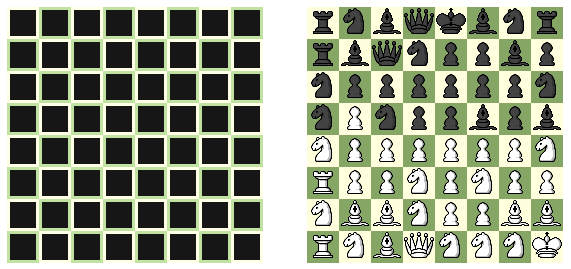
\includegraphics[width=0.9 \linewidth]{blind-allon}
\caption{What the model predicts (in single-king mode;
  Section~\ref{sec:singleking}) for {\tt 0xFFFFFFFFFFFFFFFF}, the board
  with all bits set. This is an impossible position, but it gives some
  idea of the model's biases for each square. Notably, most of the pieces
  on each half of the board have a single color. This makes sense, but
  also suggests substantial limitation. When single-king mode is off,
  the bottom right king is predicted as a white rook.} \label{fig:allon}
\end{figure}

\section{Playing blind}

Once we have predicated a board state, we can play with it. The
simplest way to do this is to use a strong chess engine to pick a move
for the position. Here, I use Stockfish with a node budget of 1
million nodes, which takes about 1 second of CPU time per move on my
computer. There are some complications:
\begin{itemize}
\item Frequently, the unblinded board will not match the true
  position, and Stockfish will choose a move that is illegal. So, as discussed
  before, we actually return a prioritized list of moves. For this first
  experiment, we just return the move Stockfish recommends, followed by all
  other moves ordered randomly.
\item Stockfish is a very strong engine, and in my opinion the code is generally
  good, but it is very sensitive to bad FEN (the notation used to give it a
  position to evaluate) strings. Given a bad string, like one that says castling
  is possible when the king isn't in its home square, often crashes the engine.
  So we need to make sure to actually pass valid positions. I accomplish this
  by making the following modifications to the predicted board:
  \begin{itemize}
  \item If a castling bit is set, but castling is not possible due to
    the position of the king or rook, clear the bit.
  \item Set the side-to-move to be the correct actual value. This uses
    the unblinded state, so is superficially cheating. But note that
    if we get the side wrong, then Stockfish's move will always be
    illegal: Moves are specified as a source and destination
    square,\footnote{Plus promotion piece. Castling is represented as
      a two-square move of the king.} and so the source square of
    Stockfish's move would always be a piece of the wrong piece's
    color. So this is equivalent to (but twice as efficient as)
    running stockfish twice, one for each side, and prioritizing the
    predicted side's move first.
  \end{itemize}
  This won't fix all positions, for example, if the white and black king are
  adjacent to one another in mutual check. If an irreparable problem is detected,
  then I just return a uniformly random move list.
\end{itemize}

It is easy to beat this chess engine, by tricking it as in
Figure~\ref{fig:trick}, although this involves unnatural moves, so it
may only apply if you know how it works.
% XXX example game?
Measuring how well it plays in an absolute sense is a subject of some
interest, so I wrote a separate paper about that~\cite{eloworld}. This
algorithm, called \verb+blind_yolo+, had an Elo World score of XXX. It
beats a purely random player with a score of 101 wins, 27 losses, and
389 draws. Making moves purely at random is one of the few fair
comparisons, since the random strategy also works with color- and
piece-blind chess.

\subsection{We three kings} \label{sec:singleking}

When evaluating the first version I found that it was predicting a
disappointingly high number of illegal positions in practice, which
was causing us to fall back on making random moves, which is mostly
boring. The second version reduces the rate of illegal positions due
to too many or too few kings~\cite{kingme}.

The model predicts a score for each type of piece in each square, and
we do not have to necessarily interpret it by always taking the
highest-scoring piece. This version first finds the two squares with
the highest scores for the white king, and same for the black king. We
take two in case the same square is predicted for both. Then this
square gets one of the kings (whichever has higher score) and the
other king goes in the highest-scoring unclaimed square. The rest of
the squares get the highest-scoring prediction as before, but we never
predict kings for them.

This change just affects the unblinding process, so we can directly
evaluate its accuracy. It gets 19.28\% of positions exactly correct
(slightly better), with an average of 3.26 piece mistakes per position
(slightly worse). This is expected; we exchange local mistakes (each
was trained independently to minimize its local error) for global
correctness (which is not taken into account at all during training).

This version, called \verb+blind_kings+, performs consistently better
than \verb+blind_yolo+ (63 wins, 45 losses, 412 draws).
% XXX could run a lot more games between these two.
% as white: 31/24/207, as black 21/32/205
It had an Elo World score of XXX.

\subsection{Spy check} \label{sec:spycheck}

Say \verb+blind_kings+ is playing as black; it remains easy to fool it
by moving black pieces into white's camp, since they are usually then
predicted to be white pieces. We can defend against this somewhat.
Since it is illegal to capture one's own piece, there is little risk
in trying; if it is indeed our own piece then the move will be
rejected, and if it is not our piece, then capturing is good for two
reasons: One, we capture a piece, and two, we avoid having
Stockfish make a move in this incorrectly predicted board. (Of course
there are many reasons why eagerly capturing a piece can be a bad
idea, but at this level of play, an edge in material is likely worth
it.)

There is one subtlety here. Above we argued that it was safe to use
the actual side-to-move instead of the predicted one; but here it
would not be equivalent to do so. Instead, we first prioritize all
apparent spy-check moves where the predicted source piece matches the
predicted side-to-move, then we try the opposite. (Ties are broken by
preferring to capture with a lower-value predicted piece, and then
randomly.) Due to this, there is some additional chance that we end up
making an especially dumb move because we both mispredicted the
side-to-move and the identity of some pieces.

(XXX evaluation here)

\subsection{Future work}

The predicted board often expresses uncertainty about some squares,
which could be thought of as probabilities. A principled improvement
would be to try to find moves that are good in expectation, that is,
integrated all possible boards in proportion to their predicted
probability. A good approximation might be had by sampling a bunch
of boards according to the predicted distribution, and then using
Stockfish to score the top $k$ moves for each; we can then order
moves by their expected score. Unfortunately, it is not easy to
efficiently get Stockfish to generate scored moves for $k \neq 1$.
Even with $k = 1$, this approach would be slow, taking about a
second for each (distinct) sampled board. So I did not try it,
at least not before submitting this paper.


\subsubsection{No, {\em u r} a lnetwork} \label{sec:legalmove}
I initially considered trying to solve this whole problem with neural
networks. The current best known engine in the world (AlphaZero) at
least {\em uses} a neural network.
% XXX is the whole thing just a network? I guessed it's probably
% alpha-beta plus a NN evaluation function?
The biggest advantage would be that it would naturally be able to
consider multiple moves under uncertainty about the board state, as
just discussed, without any particular extra logic. My plan was to
make a multiple different components that could be evaluated
separately, starting with the unblinder described, followed by a unit
that predicts legal moves, and then a unit that takes these two (and
also the 64-bit blinded mask if it likes) and scores each move.
Predicting a legal move is also a natural function for machine
learning; a move can be given just as a source and destination
square.\footnote{ There are also four choices for promotion when
  moving a pawn into the last rank. It is always the case that if any
  promotion is legal, all choices are legal, so this does not need to
  be encoded in this phase. Also, at this level of play, always
  promoting to queen is a very safe simplification.} Many pairs of
squares are always impossible (e.g. no piece can ever move from A1 to
B8); so there are only 1792 potential moves to predict. However,
training a reasonable unblinder took longer than I expected, and the
legal move predictor never really worked that well (it has a harder
job),
% (XXX some evaluation of it)
so I just settled for basing it off the single unblinder unit. Can you
do better?

\section{Conclusion}
% 
% - How do the solutions compare to other chess algorithms that
%   could be applied in the blind? Random works, also lexicographic,
%   any others? Most are inspecting the board state, obviously.
% - Could estimate the upper bound for accuracy by blinding every
%   game in the database, and doing a ``lookup''-based version of
%   the eval.

I would like to thank the little people (pawns) and the triple-blind
anonymous referrees.

% % make -j eval-unblinder.exe && ./eval-unblinder.exe net.val
% .!Evaluating model net.val...
% Loaded 50000 positions in 122.59s
% Loaded model in 0.10s
% Ran eval in 2.04s
% Reading [net.val]
% net.val: 4 layers.
% net.val: num nodes: 64 1024 12288 567 837
% net.val: indices per node/fns: 49 LEAKY_RELU 36 LEAKY_RELU 127 LEAKY_RELU 78 LEAKY_RELU
% Read from net.val.
% Invert index:
% Check it:
% ModelInfo [339885 rounds, 223224128 examples]
% Over 50000 positions:
%   9584 exactly correct (19.17%)
%   161166 piece mistakes (3.22/pos)
%   1630 castling mistakes (0.03/pos)
%   19014 move mistakes (0.38/pos)
%   181810 total mistakes (3.64/pos)
% 
% % $ make -j eval-unblinder.exe && ./eval-unblinder.exe net-before-vacuum.val
% make: 'eval-unblinder.exe' is up to date.
% Evaluating model net-before-vacuum.val...
% Loaded 50000 positions in 118.80s
% Loaded model in 3.99s
% Ran eval in 332.10s
% Reading [net-before-vacuum.val]
% net-before-vacuum.val: 4 layers.
% net-before-vacuum.val: num nodes: 64 1024 12288 567 837
% net-before-vacuum.val: indices per node/fns: 64 LEAKY_RELU 1024 LEAKY_RELU 12288 LEAKY_RELU 567 LEAKY_RELU
% Read from net-before-vacuum.val.
% Invert index:
% Check it:
% ModelInfo [146999 rounds, 9407936 examples]
% Over 50000 positions:
%   10601 exactly correct (21.20%)
%   156052 piece mistakes (3.12/pos)
%   1542 castling mistakes (0.03/pos)
%   18818 move mistakes (0.38/pos)
%   176412 total mistakes (3.53/pos)
% 
% 
% 
% without concurrent processes:
% net.val: 1.61s  (something like 1035/sec/core)
% net-before-vacuum: 229.85s (something like 7/sec/core)
% 
% 
% single_kings net.val:
% Over 50000 positions:
%   9642 exactly correct (19.28%)
%   162804 piece mistakes (3.26/pos)
%   1633 castling mistakes (0.03/pos)
%   19014 move mistakes (0.38/pos)
%   183451 total mistakes (3.67/pos)

\bibliography{chess}{}
\bibliographystyle{plain}

\end{document}
